%%%%%%%%%%%%%%%%%%%%%%%%%%%%%%%%%%%%%%%%%%%%%%%%%%%%%%%%%%%%%%%%%%%%%%%%%%%%%%%%%%%%%%%%%%%%%%
%%%%%%%%%%%%%%%%%%%%%%%%%%%%%%%%%%%%%%%%%%%%%%%%%%%%%%%%%%%%%%%%%%%%%%%%%%%%%%%%%%%%%%%%%%%%%%
%%%%%%%%%%% systemOverview
%%%%%%%%%%%%%%%%%%%%%%%%%%%%%%%%%%%%%%%%%%%%%%%%%%%%%%%%%%%%%%%%%%%%%%%%%%%%%%%%%%%%%%%%%%%%%%
%%%%%%%%%%%%%%%%%%%%%%%%%%%%%%%%%%%%%%%%%%%%%%%%%%%%%%%%%%%%%%%%%%%%%%%%%%%%%%%%%%%%%%%%%%%%%%


% \cleardoublepage
\chapter{System Overview}
\label{sec:systemOverview}

\section{Overview}
This thesis gives and overview of the the GPU implementation and performance of data aided equalizes.
but the focus of this thesis is on the computation and application of the equalizers.
Before data-aided equalizers can be computed and applied: the preambles must found, the signal packetized, the signal "de-rotated" then the channel and noise variance estimated from the de-rotated signal.
The equalizers are then computed and applied using the de-rotated signal and the estimated channel and noise variance.
After the equalizers have been applied a OQPSK detector is applied to the output of each equalizer.
A simple block Diagram is shown in Figure \ref{fig:simpleBlockDiagram}.
\begin{figure}
	\centering\includegraphics[width=6in]{figures/systemOverview/blockDiagram.pdf}
	\caption{This a simple block diagram of what the GPU does.}
	\label{fig:simpleBlockDiagram}
\end{figure}

This chapter will proceed as follows, 
section \ref{sec:preamble_detection} will explain the GPU implementation of the finding the preambles and packetizing the received signal,
section \ref{sec:frequency_offset_estimation_and_compensation} will explain the GPU implementation of estimating the frequency offset and de-rotating the signal,
section \ref{sec:channel_estimation} will explain the GPU implementation of estimating the channel,
section \ref{sec:noise_variance_estimation} will explain the GPU implementation of estimating the noise variance,
section \ref{sec:oqpsk_detector} will explain the GPU implementation of the OQPSK detector.
The explanation of the GPU implantation of the equalizers will be explained in much detail in Chapter \ref{sec:eq_eq}.





















\subsection{Preamble Detection}
\label{sec:preamble_detection}
To compute preamble assisted equalizers, estimators use the preamble to estimate various parameters. 
The details of the Preamble Detector is explained in \cite{preamble_detector}.
The iNET packet is comprised of three different sections: preamble, asynchronous marker (ASM) and the data. 
The packet and received sample structure is shown in Figure\ref{fig:packet}.
\begin{figure}
	\centering\includegraphics[width=\textwidth]{figures/gpu/packet.png}
	\caption{The iNET packet structure.}
	\label{fig:packet}
\end{figure}

The goal of the Preamble Detection step is to structure the received samples into packets or "packetize" the samples. 
To packetize, the received samples are put to into vectors with the start of each preamble as the first element.
To summarize the frame synchronization step, the preambles in the received samples are found using a preamble detector. The preamble detector output is seaching using algorithms to scan the output and find the starting index of each packet. 
Using the starting index of each packet, the received samples are packetized into vectors. 

To find the preambles in the batch, the preamble detector computs the sample correlation function between the received samples and a stored local copy of the known samples of the iNET preamble. 
A search algorithm then search the correlation function for sample indices that correlate strongest to the preamble. A spike in the correlation function indicates the start of a preamble in the received samples. 
Finally, using the starting indices of each packet, received samples are structured and synchronized into frames or packets.

The first step in the frame synchronizer is to compute the sample correlation between the received samples and the preamble.
A lower complexity preamble detector is shown in equation \eqref{eq:L-4}-\eqref{eq:L-pedone-geoghegan-4} in section \ref{sec:estimators} and repeated here for convenience.
\begin{equation}
	L(n) = \sum_{m=0}^{7}
		\left[ I^2(n,m) + Q^2(n,m) \right]
	\label{eq:gpu-L-4}
\end{equation}
where
\begin{multline}
	I(n,m) \approx \sum_{\ell\in\mathcal{L}_1}r_R(\ell+32m+n)
			- \sum_{\ell\in\mathcal{L}_2}r_R(\ell+32m+n)
			+ \sum_{\ell\in\mathcal{L}_3}r_I(\ell+32m+n)
			- \sum_{\ell\in\mathcal{L}_4}r_I(\ell+32m+n)
			\\
			+ 0.7071 \left[
				\sum_{\ell\in\mathcal{L}_5}r_R(\ell+32m+n)
				- \sum_{\ell\in\mathcal{L}_6}r_R(\ell+32m+n)
			\right. \\
			\left.
				+ \sum_{\ell\in\mathcal{L}_7}r_I(\ell+32m+n)
				- \sum_{\ell\in\mathcal{L}_8}r_I(\ell+32m+n)
			\right],
	\label{eq:gpu-L-pedone-geoghegan-2}
\end{multline}
\begin{multline}
	Q(n,m) \approx \sum_{\ell\in\mathcal{L}_1}r_I(\ell+32m+n)
			- \sum_{\ell\in\mathcal{L}_2}r_I(\ell+32m+n)
			\\
			- \sum_{\ell\in\mathcal{L}_3}r_R(\ell+32m+n)
			+ \sum_{\ell\in\mathcal{L}_4}r_R(\ell+32m+n)
			\\
			+ 0.7071 \left[
				\sum_{\ell\in\mathcal{L}_5}r_I(\ell+32m+n)
				- \sum_{\ell\in\mathcal{L}_6}r_I(\ell+32m+n)
			\right. \\
			\left.
				- \sum_{\ell\in\mathcal{L}_7}r_R(\ell+32m+n)
				+ \sum_{\ell\in\mathcal{L}_8}r_R(\ell+32m+n)
			\right]
		\label{eq:gpu-L-pedone-geoghegan-3}
\end{multline}
with
\begin{equation}
	\begin{split}
	\mathcal{L}_1 &= \{ 0, 8, 16, 24 \}\\
	\mathcal{L}_2 &= \{ 4, 20 \}\\
	\mathcal{L}_3 &= \{ 2, 10, 14, 22 \}\\
	\mathcal{L}_4 &= \{ 6, 18, 26, 30 \}\\
	\mathcal{L}_5 &= \{ 1, 7,  9, 15, 17, 23, 25, 31 \}\\
	\mathcal{L}_6 &= \{ 3, 5, 11, 12, 13, 19, 21, 27, 28, 29 \}\\
	\mathcal{L}_7 &= \{ 1, 3,  9, 11, 12, 13, 15, 21, 23 \}\\
	\mathcal{L}_8 &= \{ 5, 7, 17, 19, 25, 27, 28, 29, 31 \}.
\end{split}
\label{eq:gpu-L-pedone-geoghegan-4}
\end{equation}

The preamble detector is implemented in the GPU in two kernels as shown by the dotted box in Figure \ref{fig:preambleBlock}.
The first kernel computes the inner summations and the second computes the outer summation.
\begin{figure}
	\centering\includegraphics[width=\textwidth/10*8]{figures/gpu/preambleBlock.png}
	\caption{The block diagram for the frame synchronization implementation.}
	\label{fig:preambleBlock}
\end{figure}

The inner summation, as defined in equations \eqref{eq:gpu-L-pedone-geoghegan-2}-\eqref{eq:gpu-L-pedone-geoghegan-4}, computes an $I$ and $Q$ pair.
A single $I$ and $Q$ pair is computed by summing 32 scaled real or imaginary parts of received samples.
For each received sample an $I$ and $Q$ pair is computed.

The outer summation, as defined in equation \eqref{eq:gpu-L-4}, computes the reduced complexity maximum likelihood correlation $L$.
One sample of $L$ is computed by summing 8 squared then summed $I$ and $Q$ pairs.
For each received sample $L$ is computed.

Figure \ref{fig:L_2_packets} shows an example of the first $2\times L_{pkt} $ samples of $L$.
The local maximums in $L$ in the figure indicate a preamble starts at the maximum's sample index.
The first local maximum is at sample index $7040$, indicating the first packet starts at that index.
The figure also shows the second packet starts at sample index $19712$.
The difference between these sample indices is $ L_{pkt} $, this difference agrees with the packet length shown in Figure \ref{fig:packet}.
\begin{figure}
	\centering\includegraphics[width=5in]{figures/gpu/L_2_packets.eps}
	\caption{The output of the Preamble Detector $L(u)$.}
	\label{fig:L_2_packets}
\end{figure}

Because of the structure of the preamble, the preamble detector output $L$ has some unique properties.
The Figures in \ref{fig:L_corr_creepy} show the correlation function around an expected preamble location.
The correlation functions have peaks every 32 samples because the preamble bit sequence comprises eight repetitions of the 16-bit pattern $\text{CD98}_\text{hex}$.
The repetitive structure causes one main correlation peak with seven side peaks.

When ideal samples are received the preamble detector output looks like Figure \ref{fig:L_corr_creepy}(a).
The structure of the correlation peaks still occur when the signal to noise ratio is low, as shown in Figure \ref{fig:L_corr_creepy}(b).
But when the signal to noise ratio is low and major multipath distortion happen, the correlation peaks look like Figures \ref{fig:L_corr_creepy}(c) and (d).
The structure of the correlation peaks can cause a simple algorithm to find an incorrect preamble starting location.

In the worst case scenario, a simple algorithm might find an incorrect preamble index by searching a poorly placed search window.
A poorly placed window might search the large side correlation peaks from Figure \ref{fig:L_corr_creepy}(a) and the small main correlation peaks from Figures \ref{fig:L_corr_creepy}(c) or (d).
Because the first three side peaks in Figure \ref{fig:L_corr_creepy}(a) are much taller than the main peak in Figures \ref{fig:L_corr_creepy}(c) and (d), an incorrect preamble starting indices will result if search windows are not defined safely.
\begin{figure}
	\begin{center}
		\begin{tabular}{cc}
			\begin{minipage}[c]{3in}
				\includegraphics[width=3in]{figures/gpu/L_corr_8_clean.eps}
			\end{minipage} 
			&  
			\begin{minipage}[c]{3in}
				\includegraphics[width=3in]{figures/gpu/L_corr_8_noise.eps}
			\end{minipage} \\[12pt]
			
			\quad\quad\quad\quad(a)
			&
			\quad\quad\quad\quad(b) \\[12pt]
			
			\begin{minipage}[c]{3in}
				\includegraphics[width=3in]{figures/gpu/L_corr_17_creepy.eps}
			\end{minipage} 
			&  
			\begin{minipage}[c]{3in}
				\includegraphics[width=3in]{figures/gpu/L_corr_18_creepy.eps}
			\end{minipage} \\[12pt]
			
			\quad\quad\quad\quad(c)
			&
			\quad\quad\quad\quad(d)
			
		\end{tabular}
	\end{center}
	\caption{Detailed view of $L(u)$. 
			(a): correlation peaks of a distortion free and noiseless signal; 
			(b): correlation peaks of a distortion free but noisy signal with $E_b/N_0 = 0$dB; 
			(c): correlation peaks of a distorted and noisy signal with $E_b/N_0 = 0$dB;
			(d): correlation peaks of a distorted and noisy signal with $E_b/N_0 = 0$dB}
	\label{fig:L_corr_creepy}
\end{figure}

To prevent searching multiple preamble correlation peaks, search windows should only search the correlation peak of one preamble.
To ensure the correlation peaks from only one preamble is searched, windows of length $ L_{pkt} $ are centered on expected preamble starting locations.
Figure \ref{fig:L_windows} shows an example of safe search windows centered on expected preamble starting locations.
\begin{figure}
	\centering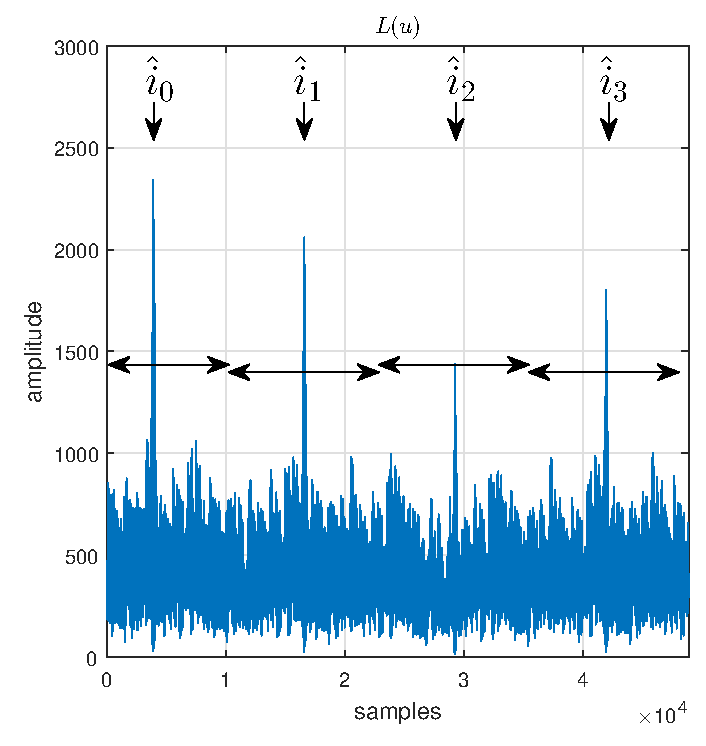
\includegraphics[width=5in]{figures/gpu/L_windows.eps}
	\caption{Safe search windows defined to search only one preamble correlation peak.}
	\label{fig:L_windows}
\end{figure}

To define safe search windows, a rough estimate of the preamble starting locations is made.
The GPU launches a kernel with one thread to search for the maximum in the first $ L_{pkt} $ samples of the received samples.
The maximum index is saved as $\hat{i}_0$.
$\hat{i}_0$ is used to make a rough estimate for all the preamble staring locations by building a vector defined as
\begin{align}
\hat{\mathbf{i}}
=     
\begin{bmatrix}
\hat{i}_0 + 0\times L_{pkt}  			\\
\hat{i}_0 + 1\times L_{pkt}  		\\
\vdots			\\
\hat{i}_0 + 3102\times L_{pkt}  		\\
\hat{i}_0 + 3103\times L_{pkt}  		
\end{bmatrix}
\label{eq:preamble_det_i_hat}
\end{align}

With rough estimates of where the preambles should be located, the GPU searches safe windows of $L$ for local maximums.
On local maximum is found in each search window by centering each window on elements from $\hat{\mathbf{i}}$.
The GPU launches one thread per search window to find the local maximum and save its sample index in $\hat{\mathbf{i}}$.
The vector $\hat{\mathbf{i}}$ has the sample indices for $3103$ local maximums that should be $ L_{pkt} $ samples apart.

Because of noise and multipath, the sample indices in $\hat{\mathbf{i}}$ are not the ideal $ L_{pkt} $ samples.
The GPU launches one thread to search $\hat{\mathbf{i}}$ for the longest chain of perfectly spaced indices.
The modulo of the last index in the longest chain of indices spaced $ L_{pkt} $ samples apart is the best estimate for $\hat{i}_0$.
Once again, $\hat{i}_0$ is updated with the best estimated first preamble starting location.
The vector $\hat{\mathbf{i}}$ is also updated again as in equation \eqref{eq:preamble_det_i_hat}. 

Now with the best estimate of the preamble starting locations, the received samples can be packetized and synchronized.
Figure \ref{fig:packets_in_batch} shows the relationship of $\hat{\mathbf{i}}$ and $\boldsymbol{r}$.
Using $\hat{\mathbf{i}}$, the GPU launches one thread per received sample to packetize $\boldsymbol{r}$ into $\boldsymbol{r}_p$ as shown in Figure \ref{fig:packetized}. The structure of $r_p$ majorly simplifies indexing and removes the need for $\hat{\mathbf{i}}$.
\begin{equation}
\boldsymbol{r}_p = 
\begin{bmatrix}
r(\hat{i}_0) 			\\
r(\hat{i}_0+1) 		\\
\vdots			\\
r(\hat{i}_0+12670)\\
r(\hat{i}_0+12671)\\
r(\hat{i}_1) 			\\
r(\hat{i}_1+1) 		\\
\vdots			\\
r(\hat{i}_{3103}+12670)\\
r(\hat{i}_{3103}+12671)\\
\end{bmatrix}
\end{equation}

\begin{figure}
	\centering\includegraphics[width=\textwidth/10*8]{figures/gpu/packets_in_batch.png}
	\caption{The starting sample index for each packet in the batch.}
	\label{fig:packets_in_batch}
\end{figure}
\begin{figure}
	\centering\includegraphics[width=\textwidth/10*8]{figures/gpu/packetized.png}
	\caption{The packetized structure of the received signals after the frame synchronization step.}
	\label{fig:packetized}
\end{figure}

The steps in Figure \ref{fig:preambleBlock} synchronize the received samples $r$ into $r_p$ by using a preamble detector.
The output of the preamble detector, $L$, is searched for local maximums.
Imperfect spacing of local maximums is fixed by finding the longest chain of perfectly spaced indices in $\hat{\mathbf{i}}$.
The received samples are then packetized based on the corrected preamble spacing.

\clearpage


\subsection{Frequency Offset Estimation and Compensation}
\label{sec:frequency_offset_estimation_and_compensation}

\subsection{Channel Estimation}
\label{sec:channel_estimation}

\subsection{Noise Variance Estimation}
\label{sec:noise_variance_estimation}

\subsection{OQPSK Detector}
\label{sec:oqpsk_detector}


%Once I Compute and apply the equalizers I need to run OQPSK demodulator or detector.
%
%This section will be asdf;lkasjf;lkas
%\begin{figure}
%	\centering\includegraphics[width=5in]{figures/systemOverview/gearPic.jpg}
%	\caption{This is our gear.}
%	\label{fig:gear_picture}
%\end{figure}
%
%
%\begin{equation}
%	L(n) = \sum_{m=0}^{7}
%		\left[ I^2(n,m) + Q^2(n,m) \right]
%	\label{eq:gpu-L-4}
%\end{equation}
%where
%\begin{multline}
%	I(n,m) \approx \sum_{\ell\in\mathcal{L}_1}r_R(\ell+32m+n)
%			- \sum_{\ell\in\mathcal{L}_2}r_R(\ell+32m+n)
%			+ \sum_{\ell\in\mathcal{L}_3}r_I(\ell+32m+n)
%			- \sum_{\ell\in\mathcal{L}_4}r_I(\ell+32m+n)
%			\\
%			+ 0.7071 \left[
%				\sum_{\ell\in\mathcal{L}_5}r_R(\ell+32m+n)
%				- \sum_{\ell\in\mathcal{L}_6}r_R(\ell+32m+n)
%			\right. \\
%			\left.
%				+ \sum_{\ell\in\mathcal{L}_7}r_I(\ell+32m+n)
%				- \sum_{\ell\in\mathcal{L}_8}r_I(\ell+32m+n)
%			\right],
%	\label{eq:gpu-L-pedone-geoghegan-2}
%\end{multline}
%\begin{multline}
%	Q(n,m) \approx \sum_{\ell\in\mathcal{L}_1}r_I(\ell+32m+n)
%			- \sum_{\ell\in\mathcal{L}_2}r_I(\ell+32m+n)
%			\\
%			- \sum_{\ell\in\mathcal{L}_3}r_R(\ell+32m+n)
%			+ \sum_{\ell\in\mathcal{L}_4}r_R(\ell+32m+n)
%			\\
%			+ 0.7071 \left[
%				\sum_{\ell\in\mathcal{L}_5}r_I(\ell+32m+n)
%				- \sum_{\ell\in\mathcal{L}_6}r_I(\ell+32m+n)
%			\right. \\
%			\left.
%				- \sum_{\ell\in\mathcal{L}_7}r_R(\ell+32m+n)
%				+ \sum_{\ell\in\mathcal{L}_8}r_R(\ell+32m+n)
%			\right]
%		\label{eq:gpu-L-pedone-geoghegan-3}
%\end{multline}
%with
%\begin{equation}
%	\begin{split}
%	\mathcal{L}_1 &= \{ 0, 8, 16, 24 \}\\
%	\mathcal{L}_2 &= \{ 4, 20 \}\\
%	\mathcal{L}_3 &= \{ 2, 10, 14, 22 \}\\
%	\mathcal{L}_4 &= \{ 6, 18, 26, 30 \}\\
%	\mathcal{L}_5 &= \{ 1, 7,  9, 15, 17, 23, 25, 31 \}\\
%	\mathcal{L}_6 &= \{ 3, 5, 11, 12, 13, 19, 21, 27, 28, 29 \}\\
%	\mathcal{L}_7 &= \{ 1, 3,  9, 11, 12, 13, 15, 21, 23 \}\\
%	\mathcal{L}_8 &= \{ 5, 7, 17, 19, 25, 27, 28, 29, 31 \}.
%\end{split}
%\label{eq:gpu-L-pedone-geoghegan-4}
%\end{equation}
%
%
%\begin{equation}
%	\hat{\omega}_0 = \frac{1}{L_q} \arg\left\{ \sum_{n=i+2L_q}^{i+7L_q-1} r(n)r^\ast(n-L_q)\right\}
%	\label{eq:jeff-ML-w-final3}
%\end{equation}
%\begin{equation}
%	\hat{\omega}_0 = \frac{1}{L_q} \arg\left\{ \mathbf{r}_{p1}^T \mathbf{r}^\ast_{p2}  \right\}.
%	\label{eq:jeff-ML-w-final3_reformed}
%\end{equation}
%where 
%\begin{align}
%\mathbf{r}_{p1}
%=     
%\begin{bmatrix}
%r_p(2L_q) 			\\
%r_p(2L_q+1) 		\\
%\vdots			\\
%r_p(7L_q - 2)\\
%r_p(7L_q - 1)
%\end{bmatrix}
%\label{eq:freq_offset_r1}
%\end{align}
%\begin{align}
%\mathbf{r}^\ast_{p2}
%=     
%\begin{bmatrix}
%r^\ast_p(L_q) 			\\
%r^\ast_p(L_q+1) 		\\
%\vdots			\\
%r^\ast_p(6L_q - 2)\\
%r^\ast_p(6L_q - 1)
%\end{bmatrix}
%\end{align}
%
%\begin{equation}
%	\hat{\mathbf{h}} = \left( \mathbf{X}^\dag\mathbf{X} \right)^{-1} \mathbf{X}^\dag\hat{\boldsymbol{\Omega}}_0^\dag \mathbf{r}
%\label{eq:jeff-ML-h-final2}
%\end{equation}
%\begin{equation}
%	\hat{\mathbf{h}} = \left( \mathbf{X}^\dag\mathbf{X} \right)^{-1} \mathbf{X}^\dag \mathbf{r}_{r1}.
%\label{eq:channel_reformed_no_freq}
%\end{equation}
%where
%\begin{align}
%\mathbf{r}_{r1}
%=     
%\begin{bmatrix}
%r_r(N_2) 		\\
%r_r(N_2+1) 		\\
%\vdots			\\
%r_r(L_p - N_1 - 2)\\
%r_r(L_p - N_1 - 1)
%\end{bmatrix}
%\end{align}
%The matrix $\mathbf{X}$ is the $(L_p+L_a-N_1-N_2)\times (N_1+N_2+1)$ convolution matrix
%formed from the iNet preamble and ASM samples. 
%The psnudo inverse of $\mathbf{X}$, $\left( \mathbf{X}^\dag\mathbf{X} \right)^{-1} \mathbf{X}^\dag$ is computed once and saved as $\mathbf{X}_{pi}$.
%Equipped with $\mathbf{X}_{pi}$ the channel estimator can be reformed again into
%\begin{equation}
%	\hat{\mathbf{h}} = \mathbf{X}_{pi} \mathbf{r}_{r1}.
%\label{eq:channel_reformed_final}
%\end{equation}
%
%
%\begin{equation}
%	\hat{\sigma}_w^2 = \frac{1}{2\rho} \left| \mathbf{r}-\hat{\boldsymbol{\Omega}}_0\mathbf{X}\hat{\mathbf{h}}\right|^2
%	\label{eq:jeff-ML-s2-final3}
%\end{equation}
%where
%\begin{equation}
%	\rho = {\rm Trace} \left\{ \mathbf{I} -  \mathbf{X}\left(\mathbf{X}^\dag\mathbf{X}\right)^{-1}\mathbf{X}^\dag \right\}.
%\end{equation}
%
%Once again, $\boldsymbol{\Omega}_0$ is included in \eqref{eq:jeff-ML-s2-final3} assuming the vector $\mathbf{r}$ has a frequency offset.
%The vector $\mathbf{r}_{r1}$ are received samples with the frequency offset compensated for, $\mathbf{r}_{r1}$ is the same vector from the channel estimator.
%The noise variance estimator is reformulated replacing $\mathbf{r}$ and removing $\boldsymbol{\Omega}_0$.
%\begin{equation}
%	\hat{\sigma}_w^2 = \frac{1}{2\rho} \left| \mathbf{r}_{r1}-\mathbf{X}\hat{\mathbf{h}}\right|^2.
%	\label{eq:noise_var_reformed}
%\end{equation}
%
%
%
%
%\begin{equation*}
%e(k)
%= 
%\begin{cases}
%0 &\text{$k$ even} \\
%\hat{a}(k-1)\mathbb{I}\{y_r(k-1)\} -  \hat{a}(k)\mathbb{R}\{y_r(k)\}  &\text{$k$ odd}\\
%\end{cases}.
%\end{equation*}
%\begin{equation}
%\hat{a}(k)= \begin{cases}
%p(k) &k<L_p+L_{asm} \\
%sgn(\mathbb{R}\{y_{r}(k)\})&k\geq L_p+L_{asm} \quad \& \quad \text{$k$ even}\\
%sgn(\mathbb{I}\{y_{r}(k)\})&k\geq L_p+L_{asm} \quad \& \quad \text{$k$ odd}\\
%\end{cases}.
%\end{equation}
%\begin{equation}
%\hat{b}(n)
%= 
%\begin{cases}
%0 &\hat{a}(n)>0 \\
%1 &\hat{a}(n)<0\\
%\end{cases}.
%\end{equation}
%
%\section{System Pictures}
%
%\section{Block Diagram}
%
%\section{Equations}
%
%\subsection{Estimators}
%\subsubsection{Preamble Detector}
%
%\subsection{Equalizers}
%
%\subsection{Decisions}
